\documentclass[12pt,a4paper]{article}
\usepackage[utf8]{inputenc}
\usepackage[english]{babel}
\usepackage{amsmath}
\usepackage{amsfonts}
\usepackage{amssymb}
\usepackage{makeidx}
\usepackage{graphicx}
\usepackage{lmodern}
\usepackage{kpfonts}
\usepackage{tikz}
\usepackage{hyperref}
\usepackage{subcaption}
\usepackage[left=2cm,right=2cm,top=4cm,bottom=2cm]{geometry}
\setlength{\parindent}{0px}
\author{Daniel Vázquez Lago}
\title{Propagación do son}
\begin{document}

\maketitle

\newpage

\tableofcontents

\newpage

\section{Objetivos:}

\begin{itemize}

\item Entender el movimiento del giroscopio, como se comporta ante determinadas fuerzas, cuales son sus aplicaciones y utilidades.

\item Nos fijaremos sobretodo en los movimientos de nutación y precesión, y cual es la relación con la frecuencia del disco. 

\item Calcularemos los momentos de inercia del disco respecto al punto de apoyo del brazo que sujeta al disco y respecto al eje del disco. 
 
\end{itemize}

\section{Descripción del movimiento de un giroscopio}
\begin{figure}[h!]
\centering
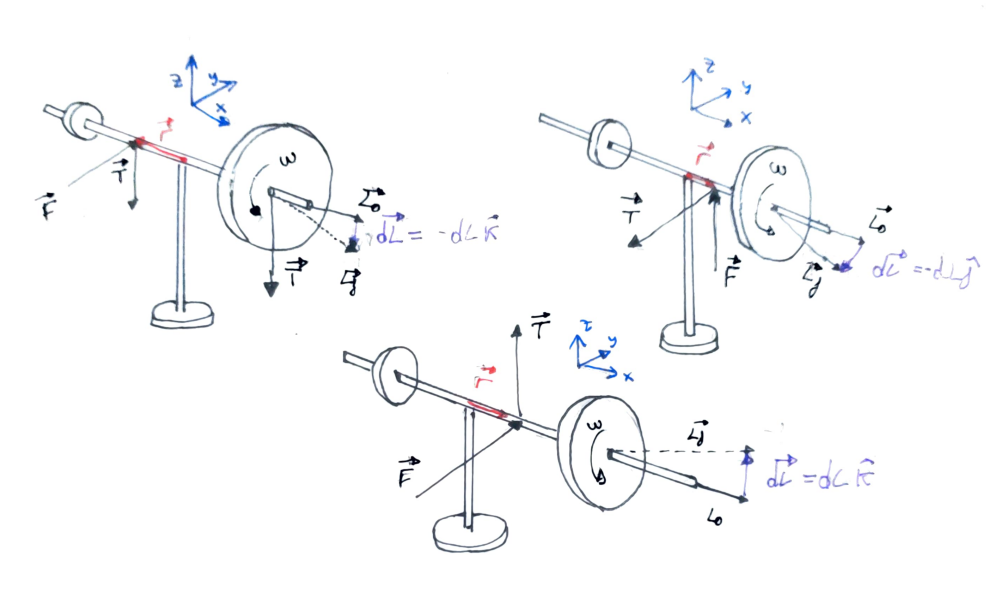
\includegraphics[scale=0.6]{xiroscopio.png}
\caption{esquema que ilustra el movimiento del giroscopio al aplicarle una fuerza para 3 casos de diferentes puntos de aplicación y dirección de la fuerza. Se puede ver que T $\perp$ L}.
\label{fig:zero}
\end{figure}

Como podemos ver en el dibujo (y experimentar en la vida real) el giroscopio se comporta de una manera un tanto rara: cuando le aplicamos una fuerza a lo largo del brazo aparece una aceleración pero en otra dirección. Esto se debe a que realmente la fuerza genera un torque que crea un momento angular respecto al punto de apoyo del brazo lo que crea un movimiento perpendicular al punto de aplicación de la fuerza y la fuerza en sí. Entonces como el momento angular total ($\vec{L}$) siempre va a tener la dirección del brazo (que en este caso la designaremos con el eje x, vector $\hat{i}$) y el punto de aplicación siempre tendrá este sentido también pues está claro que el torque que aparece siempre será perpendicular al momento angular. Además comprobamos experimentalmente que el vector torque $\vec{T}$  es paralelo al cambio infinitesimal de $\vec{L}$, por lo que $\D \vec{L} \ || \ \vec{T}$.
\section{Análisis de datos:}

\subsection{Calculo de $I_3$  directamente}

Primero medimos la altura a la que dejamos caer la pesa $m=60 \pm 1 \ g$  y el tiempo que tarda en caer la masa de tal manera que aplicando la ecuación \ref{ec:momento-incercia-3-directo} podamos extraer el momento de inercia $I_3$ (momento de inercia respecto al eje del brazo) obteniendo el valor de la pendiente del ajuste lineal ponderado (ya que las incertidumbres de $t^2$ cambian y son mucho mas grandes que las de h) $t^2 vs h$: 

\begin{equation}
h \dfrac{I_3 2}{m g r^2} = t^2 \longrightarrow I_3 = b \dfrac{m g r^2}{2}
\label{ec:momento-incercia-3-directo}
\end{equation}


\begin{figure}[h!] \centering
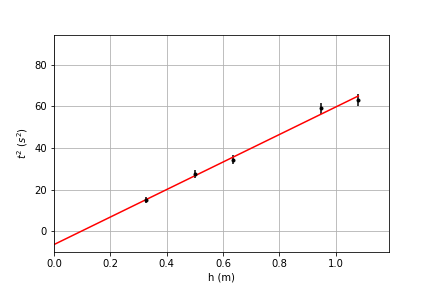
\includegraphics[scale=1]{plot-aceleracion.png}
\caption{representación gráfica de la caída, $t^2$ vs $h$}
\end{figure}

Obteniendo los siguientes datos de la regresión:

\begin{table}[h!] \centering 
\begin{tabular}{|c|c|c|c|c||c|c|} 
\hline a \ \ $(t^2)$	 & s(a)  \ \  $(t^2)$	 & b   \ \ $(m/t^2)$	 & s(b)  \ \  $(m/t^2)$ 	 & r 	 & $I_3 \ \ (kg \cdot m^2)$ 	 & s($I_3$)  $(kg \cdot m^2)$ 	 \\ \hline 
 -6.4	 & 2.1	 & 66.2	 & 3.4 	 & 0.997 & 0.0122 	 & 0.0021\\ \hline 
 \end{tabular} 
\caption{resultados de la regresión lineal y el momento de incercia $I_3$ (eq. \ref{ec:momento-incercia-3-directo})}
\end{table} 


\subsection{Calculo de $I_1$  directamente}

En este caso tenemos que calcular $I_1$ (momento de inercia respecto al punto de apoyo del brazo) a partir de un muelle y la fuerza de recuperación que ejerce. Entonces primero calculamos la  constante de recuperación y todos los datos necesarios (tab. \ref{tab:calculo-i1-directo}) y aplicando la ecuación \ref{ec:calculo-i1-directo} obtenemos $I_1$. \nocite{el valor de T es la media de 5 periodos presentes en la libreta}

\begin{equation}
w= \sqrt{\frac{2 k}{I_1}}D \longrightarrow I_1 = \dfrac{2 k T^2 D^2}{4\pi^2}
\label{ec:calculo-i1-directo}
\end{equation}

\begin{table}[h!] \centering 
\begin{tabular}{|c|c|c|c|c|c||c|c|} 
\hline $ k \ \ (kg/t^2)$ 	 & $s(k) \ \ (kg/t^2)  $	 & D  $(m)$	 & s(D) $(m)$	 & T ($s$)  & s(T)  ($s$)	 & $I_1$ 	$(kg \cdot m^2)$ & s($I_1$) 	$(kg \cdot m^2)$ \\ \hline 
 20.5	 & 3.1 	 & 0.285 	 &  0.001 	 & 0.864 & 0.011 	 & 0.0628 	 & 0.0097 \\ \hline 
 \end{tabular} 
\caption{resultados de la regresión lineal y el momento de incercia $I_3$} 
\label{tab:calculo-i1-directo}
\end{table} 



\subsection{Calculo de $I_3$ a partir del movimiento de precesión}
Cuando colgamos una pesa del extremo del brazo aparece una fuerza de dirección $-\hat{k}$ (usando el sistema de referencia de la figura \ref{fig:zero}) de tal manera que se comienza a mover con dirección $\hat{j}$. De este movimiento podemos extraer el periodo de precesión (así llamamos a este movimiento) y a partir de este la frecuencia de precesión $\Omega_p$. Conociendo esta frecuencia y la frecuencia angular media de cada vuelta podemos, a partir del cálculo de la pendiente de la regresión lineal que enfrenta $T_p$ y $w$ \ref{ec:I3-precesion} obtener $I_3$.

\begin{table}[h!] \centering
\begin{tabular}{|c|c|c||c|c|c||c|c|c|}
\hline $ w_1 $ 	 & $ \Omega_p $ 	 & $s(\Omega_p)$ 	 & $w_2$ 	 & $\Omega_p$ 	 & $s(\Omega_p)$ 	 & $w_3$ 	 & $\Omega_p$ 	 &  $s(\Omega_p)$ \\ \hline 
38.6 	 & 0.068 	 & 0.017 	 & 63.8 	 & 0.041 	 & 0.010 	 & 82.3 	 & 0.0328	 & 0.0082  \\ 
34.9 	 & 0.076 	 & 0.019 	 & 42.4 	 & 0.063 	 & 0.016 	 & 69.7 	 & 0.040 	 & 0.010  \\ 
60.0 	 & 0.047 	 & 0.017 	 & 78.9 	 & 0.0352 	 & 0.0088 	 & 56.2 	 & 0.048 	 & 0.012  \\ 
45.9 	 & 0.058 	 & 0.015 	 & 62.2 	 & 0.043 	 & 0.011 	 & 43.7 	 & 0.057 	 & 0.014  \\ 
34.2 	 & 0.077 	 & 0.019 	 & 52.8 	 & 0.053 	 & 0.013 	 & 42.1 	 & 0.059 	 & 0.015  \\ \hline
\end{tabular}
\caption{valores de la frecuencia de precesión vs velocidad angular media del disco}
\label{caca}
\end{table}

\begin{figure}[h!] \centering
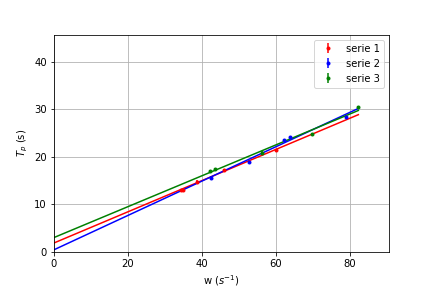
\includegraphics[scale=1]{regresionlineal-precesion.png}
\label{fig:second}
\caption{frecuencia de nutación vs velocidad angular del disco}
\end{figure}



\begin{equation}
\Omega_p=\dfrac{mgd}{I_3 w}  \longrightarrow T_p = \dfrac{2 \pi I_3}{m g d} f \longrightarrow I_3 = b \dfrac{mgd}{2 \pi} 
\label{ec:I3-precesion}
\end{equation}


Entonces como hicimos 3 series de datos obteniendo 3 regresiones lineales simples (por eso no aparece barra de error, ya que es muy pequeña) podemos extraer 3 momentos de inercia con diferente incertidumbre y realizar la media ponderada para aumentar la exactitud.

\begin{table}[h!] \centering 
\begin{tabular}{|c|c|c|c|c|c||c|c|} 
\hline  	 & $ a $  ($s$)	 & s(a) ($s$)	 & 	($s^2$) & s(b) ($s^2$)	 & r 	 & $I_3$  $(kg \cdot m^2)$	 & s($I_3$) 	$(kg \cdot m^2)$ \\ 
\hline Serie 1 	 & 1.90 	 & 0.57 	 & 0.328 	 & 0.013 	 & 0.997  & 0.0066 	 & 0.0014 \\ 
Serie 2 	 & 0.5 	 & 1.5	 & 0.361	 & 0.024	 & 0.993 	 & 0.0073 	 & 0.0016 \\ 
Serie 3 	 & 3.1 	 & 1.3	 & 0.324 	 & 0.021 	 & 0.993 	 & 0.0065 	 & 0.0014 \\ 
Media ponderada 	 & - 	 & - 	 & - 	 & - 	 & - 	 & 0.00677 	 & 0.00085 \\ 
\hline 
 \end{tabular} 
\caption{resultados de la regresión lineal y el momento de incercia $I_3$} 
\label{tab:culo}
\end{table} 


\subsection{Calculo de $I_1$ a partir del movimiento de nutación}

El movimiento de nutación se origina cuando se le da un golpe seco (fuerza instantánea) sobre el brazo de tal manera que comienza a girar sobre la dirección del momento angular original previo al golpe, como una peonza. Podemos obtener el momento de inercia $I_1$ a partir de este movimiento, tal y como refleja la ecuación \ref{ec:momento-inercia-1-nutacion}. Entonces a partir de los datos reflejados en la tabla \ref{tab:culo} podemos hacer la regresión lineal ponderada (ya que la incertidumbre del $\Omega_n$ cambia) y usando los dos momentos de inercia $I_3$ calcular dos $I_1$.


\begin{equation}
\Omega_n = \dfrac{I_3}{I_1}w  \longrightarrow I_1= \dfrac{I_3}{b} \label{ec:momento-inercia-1-nutacion}
\end{equation}

\begin{table}[h!] \centering 
\begin{tabular}{|c|c|c||c|c|c||c|c|c|}
\hline $ w_1 $ 	 & $ \Omega_n $ 	 & $s(\Omega_n)$ 	 & $w_2$ 	 & $\Omega_n$ 	 & $s(\Omega_n)$ 	 & $w_3$ 	 & $\Omega_n$ 	 &  $s(\Omega_n)$ \\ \hline 
 67.7 	 & 1.40 	 & 0.35 	 & 53.4 	 & 1.47 	 & 0.37 	 & 63.3 	 & 1.53 	 & 0.38  \\ 
 54.5 	 & 1.24	 & 0.31 	 & 65.7 	 & 1.79	 & 0.45	 & 47.3 	 & 1.14 	 & 0.28  \\ 
 42.6 	 & 1.30 	 & 0.32	 & 59.4 	 & 1.56 	 & 0.39 	 & 43.7 	 & 1.08	 & 0.27  \\ 
 29.3 	 & 0.78 	 & 0.20 	 & 50.9 	 & 1.17	 & 0.29 	 & 74.0 	 & 1.71 	 & 0.43  \\  \hline  \end{tabular}
\caption{valor de la frecuencia de una nutación vs velocidad angular media del disco} 
\end{table}


Como realizamos 3 series de las cuales podemos calcular 3 pendientes, podemos hacer la media ponderada de las 3 pendientes y así obtener una mas veraz de la cual extraer $I_1$.

\newpage

\begin{figure}[h!] \centering
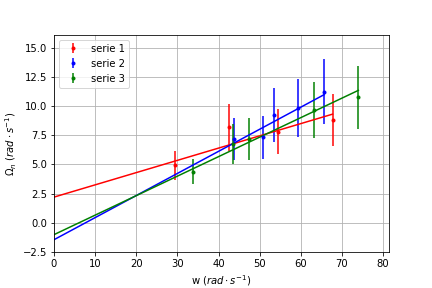
\includegraphics[scale=1]{regresionlineal-nutacion.png}
\label{fig:third}
\caption{frecuencia de nutación vs velocidad angular del disco}
\end{figure}

\begin{table}[h!] \centering 
\begin{tabular}{|c|c|c|c|c||c|c|} 
\hline  	 & $ a \ \ (s^{-1})$ 	 & $s(a) \ \  (s^{-1})$ 	 & b 	 & s(b) 	 & r 	       \\ \hline
Serie 1  & 0.35 	 & 0.42 	 & 0.0167 	 & 0.0094 	 & 0.98	  \\ 
Serie 2 	 & -0.2 	 & 1.1 	 & 0.030	 & 0.021 	 & 0.998	  \\ 
Serie 3 	 & -0.16 	 & 0.43 	 & 0.0266	 & 0.0095 	 & 0.9990 	  \\ 
Media   	 & 0.08	 & 0.29	 & 0.0223 	 & 0.0064 	 & - 	  \\ 
\hline 
 \end{tabular} 
\caption{resultados del ajuste lineal} 
\end{table} 

Entonces ahora si a partir de estos datos calculamos $I_1$ usando la ecuación \ref{ec:momento-inercia-1-nutacion} y usando tanto el $I_3$ directo como el obtenido del movimiento de precesión nos da:

$$\text{Directo:} \ I_1 \ = \ 0.087 \pm 0.029 \ kg \cdot m^2 $$
$$\text{Precesion:} \ I_1 \ = \ 0.048\pm 0.015 \ kg \cdot m^2  $$

\section{Conclusión:}

Como podemos ver hemos obtenido 3 valores para $I_1$ y 2 valores para $I_3$. Podríamos calcular los momentos de inercia teóricos pero no hemos medido la masa contrapeso para calcularla. Primero trataremos los momentos de incercia $I_3$. \\

Como se puede comprobar los 2 valores difieren mucho entre sí:
$$ I_3 \equiv 0.0122 \ (\text{directo}); \ 0.00677 \ (\text{precesión}) $$
De hecho el resultado de las medidas de la precesión son prácticamente la mitad que la calculada de forma directa. Esto es muy llamativo, y quizás no tiene mucho sentido, ya que en realidad, aun teniendo en cuenta la incertidumbre elevada debido a todos los procesos y medidas que tener en cuenta no se debería dar una diferencia tan grande. Como podemos suponer esto se tiene que dar debido a un error sistemático realizado a lo largo de la prueba la cual no debe a ver sido detectada. Si repasamos los procedimientos realizados (pesado de masas, calculo de tiempo de caida, medida de distancias...) en ninguna pudimos haber tenido un error sistemático de tal calibre menos el cálculo de la frecuencia $w$, en la que si podemos tenerla ya que dependemos de un aparato desconocido, que oscila mucho, con una sensibilidad muy grande. Para estudiar este error podríamos compararlo con el valor teórico, y quizás tomar mas valores para ver exactamente lo que ocurre y como ocurre. \\

El caso para $I_1$ es todavía más complicado, ya que ninguna de las 3 se parece realmente:

$$ I_1 \equiv 0.0628 \pm 0.0097 \ kg \cdot m^2; \ 0.087 \pm 0.029 \ kg \cdot m^2; \ 0.048  \pm 0.015 \ kg \cdot m^2  $$

Pero si que podemos observar que el valor del cálculo directo (0.0628) se encuentra a la mitad de los otros dos, además que estos tienen una incertidumbre tan grande que el intervalo abarca hasta ese valor. La incertidumbre es así de grande porque tomamos muchos valores con una incertidumbre relativamente grande. Para arreglarlo sugeriría tomar varias medidas de la frecuencia a la vez, aumentar esta (ya que cuanta mas frecuencia del disco mas estable es ante golpes y otros cambios), y quizás mejorar la forma en la que obtenemos el tiempo de nutación (ya que darle un golpe seco arbitrario, con una frecuencia media dificil de calcular y a veces con tiempos ridículos no es lo mas adecuado. De todos modos hay que decir que podría ser bastante peor, y los datos se parecen relativamente. \\

Además lo mas importante es que gracias a estos resultados y la información obtenida sobre como funciona un giroscopio (que quizás es lo mas relevante de la práctica, no tanto las similitudes entre momentos de incercia) es que podemos entender las diferentes aplicaciones del giroscopio: 

\begin{itemize}
\item Uso en cámaras de fotos: como podemos ver en la tabla \ref{caca} cuanto mayor es la frecuencia angular del disco ($w$) mayor es la frecuencia de nutación ($\Omega$), es decir, el periodo de rotación de la nutación. Si ahora consideramos un caso donde la velocidad angular del disco sea enorme, tendríamos que la rotación de la nutación sería casi inexistente. Entonces ante golpes o giros bruscos el brazo del disco se quedaría quieto. Por eso las camaras profesionales lo usan: para evitar que con golpes o movimientos bruscos se desenfoque la lente.

\item Uso en navegación: supongamos que movemos la base del giroscopio. ¿Que ocurriría?. Pues es bien sencillo: el brazo no cambiaría de dirección, seguiría apuntando hacia el mismo punto. Esto es porque no estamos aplicando ningún torque, niguna fuerza a lo largo del palo. Entonces si, por ejemplo, dejamos un giroscopio en un barco a una velocidad alta (para evitar que se pare o que haya efectos de nutación) y este comienza a inclinarse, el brazo seguirá apuntando al mismo sitio, entonces tendríamos una meidida de cuan inclinado está el barco, pudiendo tener un aviso para evitar un accidente. 
\end{itemize}

\end{document}